\documentclass{article}

\usepackage{fancyhdr}
\usepackage{extramarks}
\usepackage{amsmath}
\usepackage{amsthm}
\usepackage{amsfonts}
\usepackage{tikz}
\usepackage[plain]{algorithm}
\usepackage{algpseudocode}
\usepackage{listings} 
\usetikzlibrary{automata,positioning,positioning,calc}
\tikzset{global scale/.style={
    scale=#1,
    every node/.append style={scale=#1}
  }
}


\usepackage{color}

\definecolor{dkgreen}{rgb}{0,0.6,0}
\definecolor{gray}{rgb}{0.5,0.5,0.5}
\definecolor{mauve}{rgb}{0.58,0,0.82}

\lstset{language=Go,
  basicstyle=\ttfamily\scriptsize,
  keywordstyle=\color{blue}\ttfamily,
  stringstyle=\color{red}\ttfamily,
  commentstyle=\color{green}\ttfamily,
  breaklines,%自动换行
  }
%
% Basic Document Settings
%

\topmargin=-0.45in
\evensidemargin=0in
\oddsidemargin=0in
\textwidth=6.5in
\textheight=9.0in
\headsep=0.25in

\linespread{1.1}

\pagestyle{fancy}
\lhead{\hmwkAuthorName}
\chead{\hmwkClass\: \hmwkTitle}
\rhead{\firstxmark}
\lfoot{\lastxmark}
\cfoot{\thepage}

\renewcommand\headrulewidth{0.4pt}
\renewcommand\footrulewidth{0.4pt}

\setlength\parindent{0pt}

%
% Create Problem Sections
%

\newcommand{\enterProblemHeader}[1]{
    \nobreak\extramarks{}{Problem \arabic{#1} continued on next page\ldots}\nobreak{}
    \nobreak\extramarks{Problem \arabic{#1} (continued)}{Problem \arabic{#1} continued on next page\ldots}\nobreak{}
}

\newcommand{\exitProblemHeader}[1]{
    \nobreak\extramarks{Problem \arabic{#1} (continued)}{Problem \arabic{#1} continued on next page\ldots}\nobreak{}
    \stepcounter{#1}
    \nobreak\extramarks{Problem \arabic{#1}}{}\nobreak{}
}

\setcounter{secnumdepth}{0}
\newcounter{partCounter}
\newcounter{homeworkProblemCounter}
\setcounter{homeworkProblemCounter}{1}
\nobreak\extramarks{Problem \arabic{homeworkProblemCounter}}{}\nobreak{}

%
% Homework Problem Environment
%
% This environment takes an optional argument. When given, it will adjust the
% problem counter. This is useful for when the problems given for your
% assignment aren't sequential. See the last 3 problems of this template for an
% example.
%
\newenvironment{homeworkProblem}[1][-1]{
    \ifnum#1>0
        \setcounter{homeworkProblemCounter}{#1}
    \fi
    \section{Problem \arabic{homeworkProblemCounter}}
    \setcounter{partCounter}{1}
    \enterProblemHeader{homeworkProblemCounter}
}{
    \exitProblemHeader{homeworkProblemCounter}
}

%
% Homework Details
%   - Title
%   - Due date
%   - Class
%   - Section/Time
%   - Instructor
%   - Author
%

\newcommand{\hmwkTitle}{Assignment\ \#2}
\newcommand{\hmwkDueDate}{March 19, 2020}
\newcommand{\hmwkClass}{CSCI968 Advance Network Security}
\newcommand{\hmwkClassTime}{Assignment 2}
\newcommand{\hmwkClassInstructor}{Chen Jiageng}
\newcommand{\hmwkAuthorName}{\textbf{Mei Wangzhihui}}
\newcommand{\hmwkAuthorNum}{\textbf{2019124044}}
%
% Title Page
%

\title{
    \vspace{2in}
    \textmd{\textbf{\hmwkClass:\ \hmwkTitle}}\\
    % \normalsize\vspace{0.1in}\small{Due\ on\ \hmwkDueDate\ at 3:10pm}\\
    % \vspace{0.1in}\large{\textit{\hmwkClassInstructor\ \hmwkClassTime}}
    \vspace{3in}
}

\author{\hmwkAuthorName\ \hmwkAuthorNum}
\date{}

\renewcommand{\part}[1]{\textbf{\large Part \Alph{partCounter}}\stepcounter{partCounter}\\}

%
% Various Helper Commands
%

% Useful for algorithms
\newcommand{\alg}[1]{\textsc{\bfseries \footnotesize #1}}

% For derivatives
\newcommand{\deriv}[1]{\frac{\mathrm{d}}{\mathrm{d}x} (#1)}

% For partial derivatives
\newcommand{\pderiv}[2]{\frac{\partial}{\partial #1} (#2)}

% Integral dx
\newcommand{\dx}{\mathrm{d}x}

% Alias for the Solution section header
\newcommand{\solution}{\textbf{\large Solution}}

% Probability commands: Expectation, Variance, Covariance, Bias
\newcommand{\E}{\mathrm{E}}
\newcommand{\Var}{\mathrm{Var}}
\newcommand{\Cov}{\mathrm{Cov}}
\newcommand{\Bias}{\mathrm{Bias}}

\begin{document}

\maketitle

\pagebreak

\begin{homeworkProblem}
    \begin{center}
        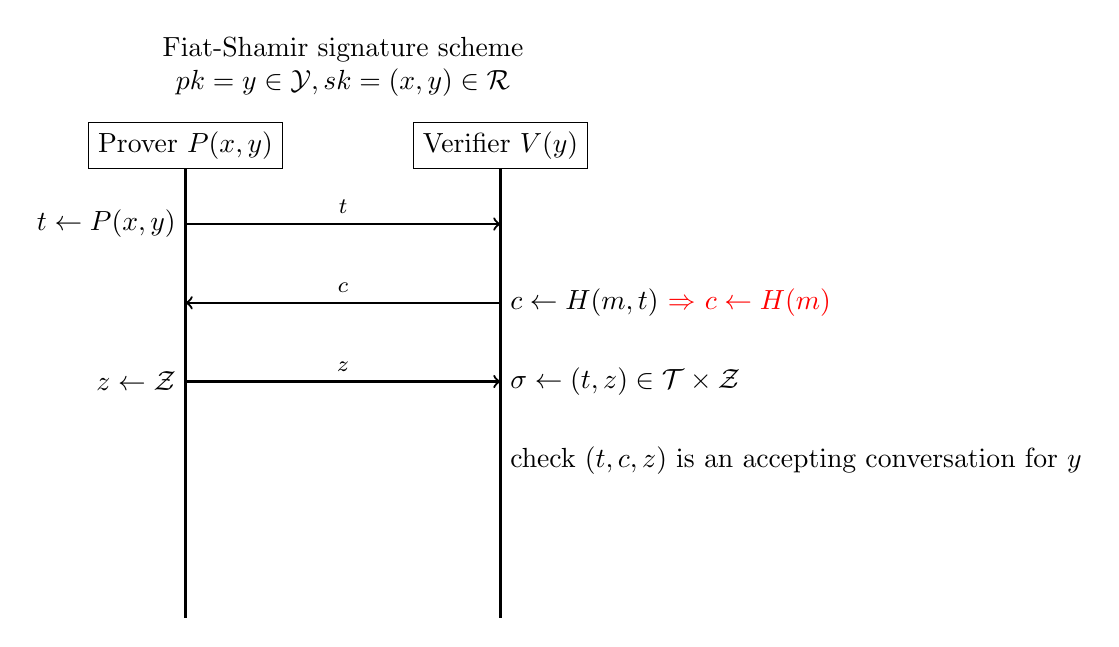
\begin{tikzpicture}
            % Public parameter:
            \node[draw=none,fill=none,align=center] (public) at (0,1) {Fiat-Shamir signature scheme \\ $pk=y\in\mathcal{Y}, sk=(x,y)\in\mathcal{R}$};
        
            % Prover
            \node[draw] (Prover) at (-2,0) {Prover $P(x,y)$};
            \draw[thick] (Prover) -- ++(0, -6);
        
            % Calculations of Prover
            \node[draw=none,fill=none,anchor=east] at ($(Prover) + (0,-1)$) {$t\leftarrow P(x,y)$};
            \node[draw=none,fill=none,anchor=east] at ($(Prover) + (0,-3)$) {$z\leftarrow \mathcal{Z}$};
        
            % Verifier
            \node[draw] (Verifier) at (2,0) {Verifier $V(y)$};
            \draw[thick] (Verifier) -- ++(0, -6);
        
            % Calculations of Verifier
            \node[draw=none,fill=none,anchor=west] at ($(Verifier) + (0,-2)$) {$c\leftarrow H(m,t) $ \textcolor{red}{$\Rightarrow$ $c\leftarrow H(m)$}};
            \node[draw=none,fill=none,anchor=west] at ($(Verifier) + (0,-3)$) {$\sigma\leftarrow(t,z)\in{\mathcal{T}\times\mathcal{Z}}$};
            \node[draw=none,fill=none,anchor=west] at ($(Verifier) + (0,-4)$) {check $(t,c,z)$ is an accepting conversation for $y$};
            % Messages
            \draw[->,thick] ($(Prover)+(0,-1)$) -- ($(Verifier)+(0,-1)$) node [pos=0.5,above,font=\footnotesize] {$t$};
            \draw[->,thick] ($(Verifier)+(0,-2)$) -- ($(Prover)+(0,-2)$) node [pos=0.5,above,font=\footnotesize] {$c$};
            \draw[->,thick] ($(Prover)+(0,-3)$) -- ($(Verifier)+(0,-3)$) node [pos=0.5,above,font=\footnotesize] {$z$};
        \end{tikzpicture}
    \end{center}
    
$t$ from prover is used to generate $c$, If the simulator has an legal pair $(t,c,z)$ it can hash any message $c_i=H(m_i)$ by itself. The $(t,c_i,z_i)$ can be accepted. It is insecure. 
   so the probability of obtaining secret key $\alpha$ is not negligible.
\end{homeworkProblem}

\begin{homeworkProblem}
    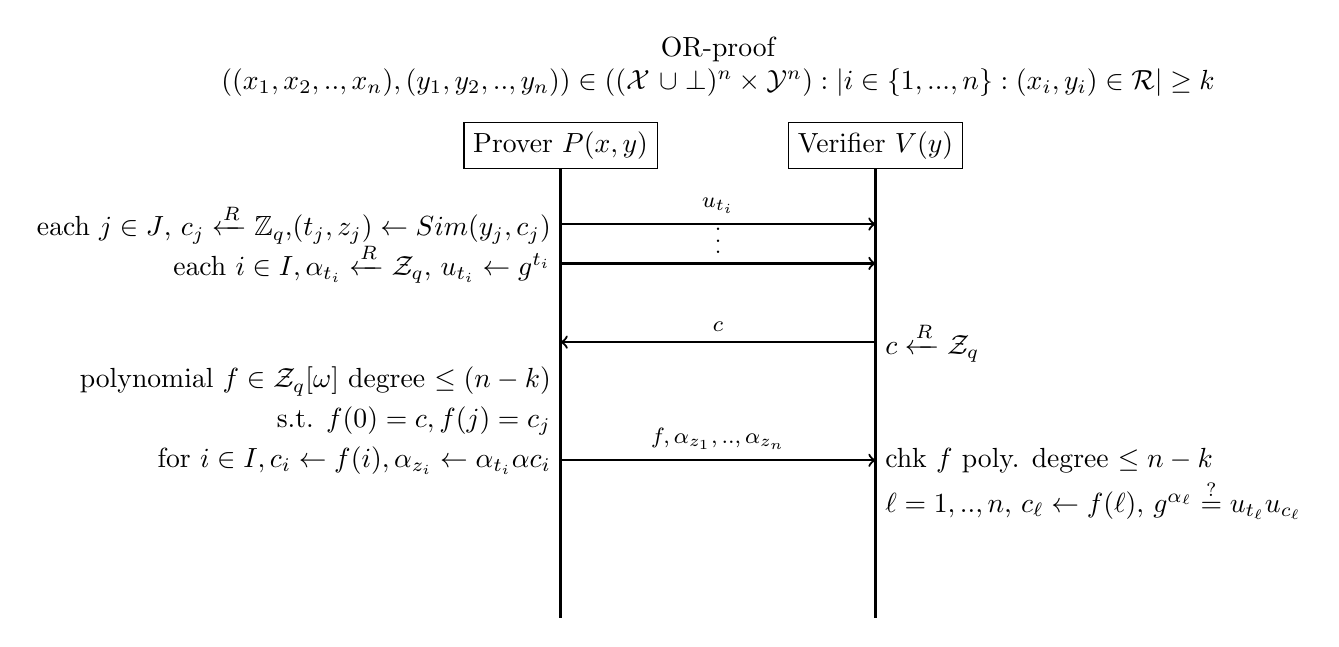
\begin{tikzpicture}[global scale=1.0]
        % Public parameter:
        \node[draw=none,fill=none,align=center] (public) at (0,1) {OR-proof \\ $((x_1,x_2,..,x_n),(y_1,y_2,..,y_n))\in((\mathcal{X}\ \cup\perp)^n\times\mathcal{Y}^n): |i\in\{1,...,n\}:(x_i,y_i)\in\mathcal{R}|\geq k$};
    
        % Prover
        \node[draw] (Prover) at (-2,0) {Prover $P(x,y)$};
        \draw[thick] (Prover) -- ++(0, -6);
        % \draw[thick] (Prover)+(-3, 0) -- ++(-3, -6) (Prover)+(-3, -6) -- ++(3, -6) (Prover)+(3, -6) -- ++(3, 0) (Prover)+(3,0) -- ++(-3,0);
        % Calculations of Prover
        \node[draw=none,fill=none,anchor=east] at ($(Prover) + (0,-1)$) {each $j\in J$, $c_j\xleftarrow{R}\mathbb{Z}_q$,$(t_j,z_j) \leftarrow Sim(y_j,c_j)$};
        \node[draw=none,fill=none,anchor=east] at ($(Prover) + (0,-1.5)$) {each $i\in I, \alpha_{t_i}\xleftarrow{R}\mathcal{Z}_q$, $u_{t_i}\leftarrow g^{t_i}$};
        \node[draw=none,fill=none,anchor=east] at ($(Prover) + (0,-3)$) { polynomial $f\in\mathcal{Z}_q[\omega]$ degree $\leq(n-k)$};
        \node[draw=none,fill=none,anchor=east] at ($(Prover) + (0,-3.5)$) {s.t. $f(0)=c,f(j)=c_j$};
        \node[draw=none,fill=none,anchor=east] at ($(Prover) + (0,-4.0)$) {for $i\in I,c_i\leftarrow f(i),\alpha_{z_i}\leftarrow\alpha_{t_i}\alpha{c_i}$};
        % Verifier
        \node[draw] (Verifier) at (2,0) {Verifier $V(y)$};
        \draw[thick] (Verifier) -- ++(0, -6);
    
        % Calculations of Verifier
        \node[draw=none,fill=none,anchor=west] at ($(Verifier) + (0,-2.5)$) {$c \xleftarrow{R}\mathcal{Z}_q$};
        \node[draw=none,fill=none,anchor=west] at ($(Verifier) + (0,-3)$) {};
        \node[draw=none,fill=none,anchor=west] at ($(Verifier) + (0,-4)$) { chk $f$ poly. degree $\leq n-k$};
        \node[draw=none,fill=none,anchor=west] at ($(Verifier) + (0,-4.5)$) {$\ell=1,..,n$, $c_\ell\leftarrow f(\ell)$, $g^{\alpha_{\ell}}\overset{?}{=}u_{t_\ell}u_{c_{\ell}}$};
        % Messages
        \draw[->,thick] ($(Verifier)+(0,-2.5)$) -- ($(Prover)+(0,-2.5)$) node [pos=0.5,above,font=\footnotesize] {$c$};
        \draw[->,thick] ($(Prover)+(0,-1)$) -- ($(Verifier)+(0,-1)$) node [pos=0.5,above,font=\footnotesize] {$u_{t_i}$};
        \draw[->,thick] ($(Prover)+(0,-1.5)$) -- ($(Verifier)+(0,-1.5)$) node [pos=0.5,above,font=\footnotesize] {\vdots};
        \draw[->,thick] ($(Prover)+(0,-4.0)$) -- ($(Verifier)+(0,-4.0)$) node [pos=0.5,above,font=\footnotesize] {$f,\alpha_{z_1},..,\alpha_{z_n}$};
    \end{tikzpicture}
\end{homeworkProblem}
\begin{homeworkProblem}
    \begin{center}
        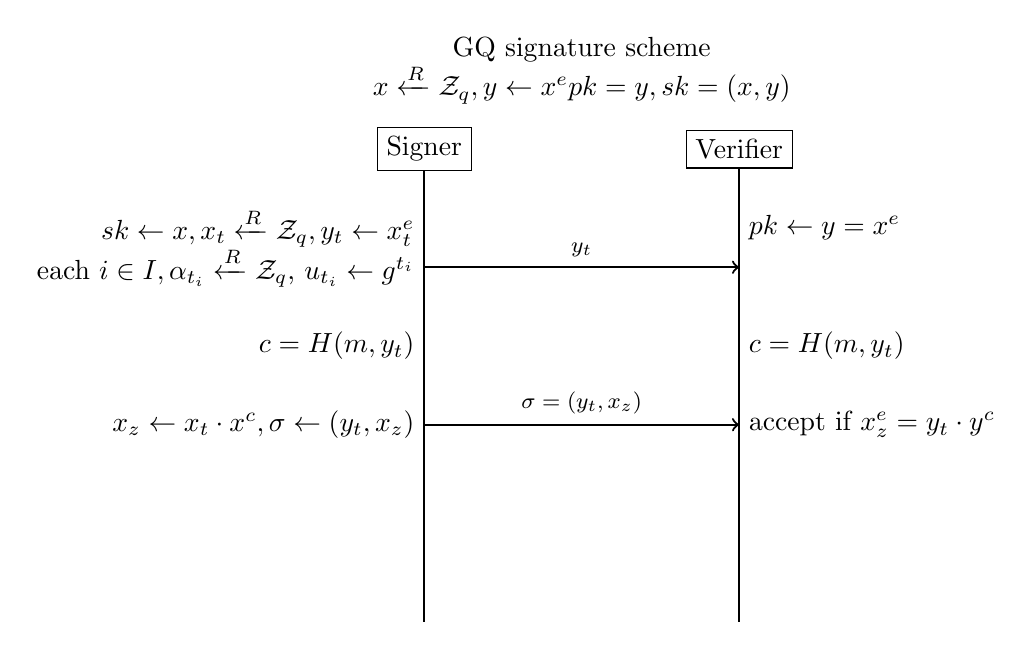
\begin{tikzpicture}[global scale=1.0]
            % Public parameter:
            \node[draw=none,fill=none,align=center] (public) at (0,1) {GQ signature scheme \\ $x\xleftarrow{R}\mathcal{Z}_q,y\leftarrow x^e pk=y, sk=(x,y)$};
        
            % Signer
            \node[draw] (Signer) at (-2,0) {Signer};
            \draw[thick] (Signer) -- ++(0, -6);
            % \draw[thick] (Signer)+(-3, 0) -- ++(-3, -6) (Signer)+(-3, -6) -- ++(3, -6) (Signer)+(3, -6) -- ++(3, 0) (Signer)+(3,0) -- ++(-3,0);
            % Calculations of Signer
            \node[draw=none,fill=none,anchor=east] at ($(Signer) + (0,-1)$) {$sk\leftarrow x,x_t\xleftarrow{R}\mathcal{Z}_q,y_t\leftarrow x_t^e $};
            \node[draw=none,fill=none,anchor=east] at ($(Signer) + (0,-1.5)$) {each $i\in I, \alpha_{t_i}\xleftarrow{R}\mathcal{Z}_q$, $u_{t_i}\leftarrow g^{t_i}$};
            \node[draw=none,fill=none,anchor=east] at ($(Signer) + (0,-2.5)$) { $c=H(m,y_t)$};
            \node[draw=none,fill=none,anchor=east] at ($(Signer) + (0,-3.5)$) {$x_z\leftarrow x_t\cdot x^c, \sigma\leftarrow(y_t,x_z)$};
            % Verifier
            \node[draw] (Verifier) at (2,0) {Verifier};
            \draw[thick] (Verifier) -- ++(0, -6);
        
            % Calculations of Verifier
            \node[draw=none,fill=none,anchor=west] at ($(Verifier) + (0,-1)$) {$pk\leftarrow y=x^e$};
            \node[draw=none,fill=none,anchor=west] at ($(Verifier) + (0,-2.5)$) {$c=H(m,y_t)$};
            \node[draw=none,fill=none,anchor=west] at ($(Verifier) + (0,-3.5)$) {accept if $x_z^e=y_t\cdot y^c$};
            % Messages
            \draw[->,thick] ($(Signer)+(0,-1.5)$) -- ($(Verifier)+(0,-1.5)$) node [pos=0.5,above,font=\footnotesize] {$y_t$};
            \draw[->,thick] ($(Signer)+(0,-3.5)$) -- ($(Verifier)+(0,-3.5)$) node [pos=0.5,above,font=\footnotesize] {$\sigma=(y_t,x_z)$};
        \end{tikzpicture}
    \end{center}
    \begin{center}
        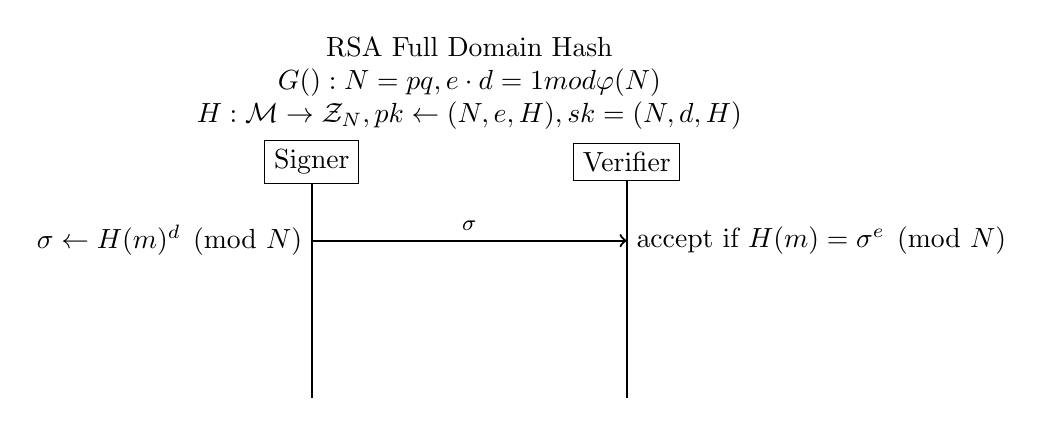
\begin{tikzpicture}[global scale=1.0]
            % Public parameter:
            \node[draw=none,fill=none,align=center] (public) at (0,1) {RSA Full Domain Hash \\ $G(): N=pq, e\cdot d=1 mod{\varphi(N)}$ \\ $H: \mathcal{M} \rightarrow \mathcal{Z}_N,pk\leftarrow(N,e,H), sk=(N,d,H)$};
             % Signer
             \node[draw] (Signer) at (-2,0) {Signer};
             \draw[thick] (Signer) -- ++(0, -3);
             
            % Calculations of Signer
            \node[draw=none,fill=none,anchor=east] at ($(Signer) + (0,-1)$) {$\sigma\leftarrow H(m)^d\pmod{N}$};
            
            % Verifier
            \node[draw] (Verifier) at (2,0) {Verifier};
            \draw[thick] (Verifier) -- ++(0, -3);
        
            % Calculations of Verifier
            \node[draw=none,fill=none,anchor=west] at ($(Verifier) + (0,-1)$) {accept if $H(m)=\sigma^e\pmod{N}$};
    
            % Messages
            \draw[->,thick] ($(Signer)+(0,-1)$) -- ($(Verifier)+(0,-1)$) node [pos=0.5,above,font=\footnotesize] {$\sigma$};
        \end{tikzpicture}
    \end{center}

    Fiat-Shamir heuristic GQ signature doesn't need the involvement of d, thus no need of computing it. The Fiat-Shamir heuristic GQ signature is more efficient than 

\end{homeworkProblem}
\end{document}
